% Statistical Estimation of Canteen Arrival Overload Probability Using Poisson Distribution
% IEEE conference format (IEEEtran). Build:  python paper/make_figures.py && cd paper && latexmk -pdf canteenflow_ieee.tex
\documentclass[conference,a4paper]{IEEEtran}
\IEEEoverridecommandlockouts

\usepackage[T1]{fontenc}
\usepackage{amsmath}
\usepackage{graphicx}
\usepackage{booktabs}
\usepackage{array}
\usepackage{cite}
\usepackage{url}
\usepackage{xcolor}
\usepackage{tikz}
\usetikzlibrary{positioning,arrows.meta}
\usepackage[hidelinks]{hyperref}

\graphicspath{{figures/}}
\makeatletter
\newcommand{\tablerows}[1]{\@@input #1 }  % primitive \input, safe inside tabular before \bottomrule
% start a new, centred row of author blocks (IEEEtran otherwise left-aligns a lone fourth author)
\newcommand{\linebreakand}{\end{@IEEEauthorhalign}\hfill\mbox{}\par\mbox{}\hfill\begin{@IEEEauthorhalign}}
\makeatother
\definecolor{ink}{HTML}{1B2A4A}
\definecolor{teal}{HTML}{00868B}
\definecolor{soft}{HTML}{E3F4F4}

\begin{document}

\title{Statistical Estimation of Canteen Arrival Overload Probability Using Poisson Distribution}

\author{
\IEEEauthorblockN{Faraz Akhtar Khan}
\IEEEauthorblockA{\textit{School of Computer Science}\\
\textit{Engineering and Information Systems}\\
\textit{Vellore Institute of Technology}\\
Vellore, India}
\and
\IEEEauthorblockN{Mayur Krishna}
\IEEEauthorblockA{\textit{School of Computer Science}\\
\textit{Engineering and Information Systems}\\
\textit{Vellore Institute of Technology}\\
Vellore, India}
\and
\IEEEauthorblockN{Malhar Bhosale}
\IEEEauthorblockA{\textit{School of Computer Science}\\
\textit{Engineering and Information Systems}\\
\textit{Vellore Institute of Technology}\\
Vellore, India}
\linebreakand
\IEEEauthorblockN{Manimaran A}
\IEEEauthorblockA{\textit{School of Advanced Sciences}\\
\textit{Vellore Institute of Technology}\\
Vellore, India}
}

\maketitle

\begin{abstract}
University canteens see sharp, short-lived rises in arrivals during the lunch peak, and the practical question for
students and managers is how likely a given time slot is to exceed what the serving counters can handle. This paper
models student arrivals in each 15-minute slot as a Poisson count, estimates a separate rate $\lambda_t$ for every slot
with an exact confidence interval, tests the Poisson assumption slot by slot, and converts the tail probability
$P(X_t > C)$ into low, medium and high overload-risk labels. The analysis is then extended from description to
prediction: a multiple linear regression on log counts gives day-specific rates for each day of the week; a
Poisson--Gamma mixture tests for extra day-to-day variation; Monte Carlo simulation gives the probability that each slot
is the day's peak; and Bayes' theorem with a Gamma prior provides a same-day update. Every forecast is checked on days
the model has not seen with a rolling one-day-ahead backtest. On 40 days of recorded lunch-time arrivals, the
riskiest slot is 12:45--13:00 ($P = 55.9\%$ at $C = 30$), 13:00--13:15 is significantly quieter, weekends bring about
26\% fewer arrivals, and on a regular Monday the peak falls in 12:30--13:00 with probability 83\%. On 20 unseen days
the busiest slot was named correctly 60\% of the time against 40\% by chance and the overload forecasts had a Brier
skill of 31\% over a per-slot average, while the gain in point accuracy was not statistically significant. All methods
use standard probability and statistics, and the implementation is released as an interactive dashboard.
\end{abstract}

\begin{IEEEkeywords}
Poisson distribution, arrival process, overload probability, peak-time forecasting, Bayesian updating,
negative binomial, hypothesis testing, university canteen.
\end{IEEEkeywords}

% ===================================================================================================
\section{Introduction}
University canteens experience changing arrival intensity during lunch. When more students arrive in a short interval
than the counters can serve, queues form, the dining area becomes crowded and popular dishes run out. Decisions about
when to eat, how many counters to open and when to stagger breaks are usually taken by intuition rather than from
measured arrival behaviour.

Existing canteen studies treat the canteen as a complete system. Tang \textit{et al.}~\cite{tang2019a} collected
camera data at a university canteen and built a pedestrian-flow model of the whole meal process, and a cellular-automaton
model followed~\cite{tang2019b}. Queueing studies set the number of serving windows from assumed Poisson
arrivals~\cite{chen2011,yuan2023,jiao2022}. These models are valuable but heavy, and they leave a simple question
unanswered: \textit{what is the probability that arrivals exceed a chosen level during a particular time slot, and
when will today's peak occur?}

This paper answers that question with standard probability and statistics. Its contributions are:
\begin{enumerate}
\item A per-slot Poisson model of canteen arrivals with exact confidence intervals, slot-by-slot goodness-of-fit and
dispersion tests, and an overload probability $P(X_t > C)$ mapped to risk labels.
\item A day-specific forecast of slot rates by multiple linear regression on day-of-week and day-type indicators,
with a Poisson--Gamma model for day-to-day variation.
\item The probability that each slot is the day's peak, obtained by simulation, and a Bayesian update of the
rest-of-day forecast from the counts observed so far.
\item A validation protocol that forecasts each day from earlier days only and tests the forecasts with proportion,
paired, sign, Kolmogorov--Smirnov and chi-square tests, and the Brier score.
\end{enumerate}
The methods are applied to 40 days of recorded arrival counts at a university canteen (Section~\ref{sec:data}).

The rest of the paper is organised as follows. Section~\ref{sec:related} reviews related work and the gaps it leaves.
Section~\ref{sec:data} describes the data and Section~\ref{sec:method} the methodology. Section~\ref{sec:results}
presents results, Section~\ref{sec:discussion} discusses them and their limitations, and Section~\ref{sec:conclusion}
concludes.

% ===================================================================================================
\section{Related Work}\label{sec:related}

\subsection{Canteen flow and queueing}
Tang \textit{et al.}~\cite{tang2019a} counted arrivals and departures in 5-minute segments at a Beihang University
canteen between 10:30 and 13:30 and calibrated a model of window choice, movement, congestion delay and meal duration.
They note that arrivals follow a Poisson distribution within short periods with a rate that changes every few minutes,
and that days differ with the class timetable; the arrival rate, however, is an input to their simulation rather than a
quantity that is tested or predicted. Queueing studies set windows, seats and opening times with M/M/$n$/$m$ and
M/M/$C$ models~\cite{chen2011,yuan2023}; Jiao \textit{et al.}~\cite{jiao2022} simulate one constant arrival rate of
19.3 students per minute and find seven windows optimal. In all of these the Poisson arrival assumption is an input,
not a finding.

\subsection{Testing Poisson arrivals}
Brown \textit{et al.}~\cite{brown2005} established a statistical treatment of service arrivals and a test that a point
process is Poisson. Kim and Whitt~\cite{kim2014} show that nonhomogeneous Poisson models fit call-centre and hospital
arrivals only after careful analysis: long subintervals and pooled days create overdispersion. Green
\textit{et al.}~\cite{green2007} show that time-varying demand needs short, piecewise-constant rates, and
Leemis~\cite{leemis1991} estimates such rates from repeated days. Cameron and Trivedi~\cite{cameron1990} give tests for
overdispersion in Poisson models.

\subsection{Forecasting arrival rates}
Weinberg \textit{et al.}~\cite{weinberg2007} forecast within-day call-centre rates as a daily level times a weekday
shape and update the forecast during the day; Shen and Huang~\cite{shen2008} forecast quarter-hour Poisson rate
profiles and report that intraday updating cut staffing error by 14.5\%. Aldor-Noiman \textit{et al.}~\cite{aldornoiman2009}
add special-event indicators and compare against an ``industry model'' that averages past slots, which is the
per-slot average used by descriptive canteen analyses. Matteson \textit{et al.}~\cite{matteson2011} stress that small
hourly counts should be modelled as Poisson directly rather than through normal approximations. Ibrahim
\textit{et al.}~\cite{ibrahim2016} survey the field: arrivals are overdispersed and correlated within a day, which a
Gamma ``busyness factor'' captures, and simple fixed-effect models are hard to beat.

\subsection{Campus dining and forecast verification}
Shah \textit{et al.}~\cite{shah2025} forecast daily customer totals in a university self-service restaurant with
machine learning, although their own data show strong hourly peaks; Variskhanov and Arreeras~\cite{variskhanov2026}
issue a day-level ``early peak'' badge from Wi-Fi telemetry. For probability forecasts of a yes/no event, the Brier
score~\cite{brier1950} and a skill score against a reference forecast~\cite{mcnulty1988} are the standard checks.

\subsection{Research gaps}
Table~\ref{tab:gaps} summarises what the reviewed work leaves open. Four gaps motivate this paper:
(G1)~no per-slot overload probability for a canteen; (G2)~the Poisson assumption is built in rather than tested;
(G3)~no prediction of a specific day's rates or of the peak time, with or without the day's early counts; and
(G4)~no test of canteen forecasts on unseen days. These are gaps of focus and application, not a claim that Poisson
modelling of arrivals is new.

\begin{table}[t]
\caption{Representative studies and what they leave open}\label{tab:gaps}
\centering\footnotesize
\begin{tabular}{@{}>{\raggedright\arraybackslash}p{0.26\columnwidth}>{\raggedright\arraybackslash}p{0.29\columnwidth}>{\raggedright\arraybackslash}p{0.35\columnwidth}@{}}
\toprule
Study & Approach & Left open for this work \\
\midrule
Tang \textit{et al.}~\cite{tang2019a} & Pedestrian-flow model of a canteen & Arrival rate is an input; no slot overload probability \\
Jiao \textit{et al.}~\cite{jiao2022} & M/M/$C$ simulation, one rate & Poisson assumed; rate constant all lunch \\
Kim \& Whitt~\cite{kim2014} & Tests of Poisson arrivals & Call centres and hospitals, not canteens \\
Weinberg \textit{et al.}~\cite{weinberg2007}, Shen \& Huang~\cite{shen2008} & Rate forecasting, intraday update & Large-count approximations; staffing, not overload \\
Shah \textit{et al.}~\cite{shah2025} & ML forecast of campus dining & Daily totals only; no probabilities \\
\bottomrule
\end{tabular}
\end{table}

% ===================================================================================================
\section{Data}\label{sec:data}
\textit{Recorded arrivals.} Student arrivals at the canteen were recorded in fixed 15-minute slots covering the start
of the lunch period, 12:30--13:15 (three slots), on 40 consecutive days from 5~January to 13~February 2026. The record
includes weekends: 30 weekdays and 10 Saturdays and Sundays, marked with the day type ``Weekend''. Each record holds the
date, the weekday, the day type, the slot and the number of students who entered in that slot, in the style of the
interval counts of~\cite{tang2019a}.

\textit{Cleaning.} Missing, negative, fractional, unreadable and duplicate counts are dropped rather than imputed,
because imputing the mean would shrink the variance and bias the dispersion test. All 120 records passed these checks,
giving 120 slot observations (40 per slot). Counts range from 17 to 41 students per slot, with a mean of 30.0.

% ===================================================================================================
\section{Methodology}\label{sec:method}
Fig.~\ref{fig:framework} shows the nine-step framework. Steps 1--7 estimate and check overload risk; steps 8--9 forecast
and validate.

\begin{figure}[t]
\centering
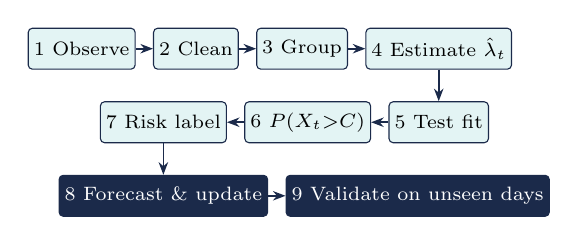
\begin{tikzpicture}[node distance=2.2mm, every node/.style={font=\scriptsize},
  box/.style={draw=ink, fill=soft, rounded corners=1.5pt, minimum height=5.2mm, inner sep=2pt, align=center},
  fbox/.style={box, fill=ink, text=white}, arr/.style={-{Stealth[length=1.6mm]}, ink, semithick}]
\node[box] (a) {1 Observe};
\node[box, right=of a] (b) {2 Clean};
\node[box, right=of b] (c) {3 Group};
\node[box, right=of c] (d) {4 Estimate $\hat\lambda_t$};
\node[box, below=4mm of d] (e) {5 Test fit};
\node[box, left=of e] (f) {6 $P(X_t{>}C)$};
\node[box, left=of f] (g) {7 Risk label};
\node[fbox, below=4mm of g] (h) {8 Forecast \& update};
\node[fbox, right=of h] (i) {9 Validate on unseen days};
\draw[arr] (a)--(b); \draw[arr] (b)--(c); \draw[arr] (c)--(d); \draw[arr] (d)--(e);
\draw[arr] (e)--(f); \draw[arr] (f)--(g); \draw[arr] (g)--(h); \draw[arr] (h)--(i);
\end{tikzpicture}
\caption{Statistical framework. Light boxes: estimation and checking; dark boxes: prediction and validation.}
\label{fig:framework}
\end{figure}

\subsection{Poisson model and estimation}
Let $X_t$ be the number of students arriving in slot $t$. The model assumes
\begin{equation}
X_t \sim \mathrm{Poisson}(\lambda_t),\qquad P(X_t = x) = \frac{e^{-\lambda_t}\lambda_t^{x}}{x!},
\end{equation}
$x = 0, 1, 2, \dots$, with $E[X_t] = \mathrm{Var}(X_t) = \lambda_t$.
For slot $t$ observed on $m$ days with counts $x_1,\dots,x_m$, the maximum-likelihood estimate is the sample mean
$\hat\lambda_t = \sum x_i / m$. Because $S = \sum x_i \sim \mathrm{Poisson}(m\lambda_t)$, the exact (Garwood) interval
is~\cite{garwood1936}
\begin{equation}
\left[\frac{\chi^2_{\alpha/2}(2S)}{2m},\ \frac{\chi^2_{1-\alpha/2}(2S+2)}{2m}\right].
\end{equation}

\subsection{Checking the Poisson assumption}
Two tests are applied to every slot at $\alpha = 0.05$. The index-of-dispersion test uses
$D = (m-1)s^2/\bar x \sim \chi^2_{m-1}$ under $H_0$, two-sided. The chi-square goodness-of-fit test compares observed
and expected frequencies, $\chi^2 = \sum_i (O_i - E_i)^2/E_i$ with $k-2$ degrees of freedom, after merging adjacent
counts until every expected frequency is at least 5~\cite{cochran1954}. Because $K$ slots are tested, the number of
rejections is compared with a Binomial$(K, \alpha)$ distribution.

\subsection{Overload probability and risk}
With capacity $C$ per slot (threshold $K = C+1$),
\begin{equation}
P(X_t > C) = 1 - \sum_{x=0}^{C}\frac{e^{-\hat\lambda_t}\hat\lambda_t^{x}}{x!}.
\end{equation}
A slot is labelled low risk below 20\%, high risk above 50\% and medium otherwise; these thresholds are project
decision rules. The probability is also evaluated at both ends of the confidence interval for $\lambda_t$, and the
smallest capacity keeping it below a target is reported for planning. To check that the quietest slot is genuinely
quieter than the runner-up, the exact conditional test
$S_1 \mid (S_1 + S_2) \sim \mathrm{Binomial}(S_1+S_2, m_1/(m_1+m_2))$ is used~\cite{przyborowski1940}.

\subsection{Day-specific rates by regression}
To predict a particular day, the slot rate is allowed to depend on the day of the week $d$ and the day type $e$. Multiple
linear regression with dummy variables is fitted by least squares to log counts:
\begin{equation}
\ln(x_{dt} + 0.5) = \beta_0 + \alpha_t + \gamma_d + \delta_e + \varepsilon_{dt},
\end{equation}
with 12:30 and Monday as reference levels; a day type that coincides with whole days of the week (here the weekend,
which is exactly Saturday and Sunday) is captured by those day terms and gets no separate coefficient. Each
coefficient is tested with
$t_j = \hat\beta_j/\mathrm{SE}(\hat\beta_j) \sim t_{n-p}$, and fitted values are returned to the count scale with
Duan's smearing factor $\overline{e^{\hat\varepsilon}}$~\cite{duan1983}. Weekday effects on daily totals are also
tested with one-way ANOVA and the Kruskal--Wallis test, and weekends against weekdays with Welch's $t$-test and the
Mann--Whitney $U$ test~\cite{johnson2018}.

\subsection{Day-to-day variation: Poisson--Gamma model}
Whole days can be busier or quieter than predicted~\cite{ibrahim2016}. Let each day carry a busyness factor
$W \sim \mathrm{Gamma}(1/v, 1/v)$ with mean 1 and variance $v$. By the theorem of total probability,
\begin{equation}
P(X_t = x) = \int_0^\infty \frac{e^{-w\lambda_t}(w\lambda_t)^x}{x!}\, g(w)\,dw ,
\end{equation}
a negative binomial with $E[X_t] = \lambda_t$ and $\mathrm{Var}(X_t) = \lambda_t + v\lambda_t^2$. The Pearson statistic
$\chi^2_P = \sum (x - \hat\lambda)^2/\hat\lambda$ follows $\chi^2_{n-p}$ under the plain Poisson model, and its excess
gives the moment estimate $\hat v = (\chi^2_P - (n-p))/\sum\hat\lambda$~\cite{cameron1990}. With $v = 0$ the model
reduces to the Poisson model above.

\subsection{Peak-time probability}
For a chosen day, $N = 20{,}000$ lunch periods are simulated: draw $W$, then $X_t \sim \mathrm{Poisson}(W\hat\lambda_t)$
independently for each slot. The share of simulated days on which slot $t$ has the largest count (ties broken at
random) estimates $P(\text{slot } t \text{ is the peak})$; the same draws give $P(\text{at least one slot exceeds } C)$.

\subsection{Same-day Bayesian update}
After the first $k$ slots of today have been counted, Bayes' theorem with the Gamma prior $W \sim \mathrm{Gamma}(a, a)$,
$a = 1/v$, gives the conjugate posterior
\begin{equation}
W \mid x_1,\dots,x_k \sim \mathrm{Gamma}\Big(a + \sum_{t\le k} x_t,\ a + \sum_{t\le k}\hat\lambda_t\Big),
\end{equation}
and each later slot then has a negative binomial predictive distribution, which yields the updated $P(X_t > C)$.

\subsection{Validation on unseen days}
The first half of the record (20 days) is used for training; each later day is forecast from all earlier days only
and compared with what happened. The model is
compared with the per-slot average used in descriptive analyses (the ``industry model''~\cite{aldornoiman2009}). The
checks are: coverage of 95\% prediction intervals ($z$-test of a proportion); whether the predicted busiest slot is
correct more often than chance (one-sided $z$-test); daily mean absolute error against the baseline (paired $t$-test
and sign test); calibration of the full forecast distribution through randomised probability integral transform (PIT)
values, $u = F(x-1) + V[F(x) - F(x-1)]$ with $V \sim U(0,1)$, tested for uniformity by Kolmogorov--Smirnov and
chi-square tests; and the Brier score $B = \frac1N\sum (p_i - o_i)^2$ of the overload forecasts with skill
$1 - B_\text{model}/B_\text{baseline}$~\cite{brier1950,mcnulty1988}. Spearman rank correlation between consecutive
slots and a Wald--Wolfowitz runs test on daily residual signs check within-day and day-to-day dependence.

\subsection{Implementation}
The methods are implemented in Python with NumPy, pandas and SciPy, covered by 72 automated tests, and presented in an
interactive Streamlit dashboard whose home page answers ``when should I go?'' in plain language. All figures and tables
in this paper are generated from the same code.

% ===================================================================================================
\section{Results}\label{sec:results}
All results use the 40 recorded days, capacity $C = 30$ per slot and $\alpha = 0.05$.

\subsection{Arrival rates and model fit}
The arrival rate is 30.5 at 12:30--12:45, peaks at 31.5 at 12:45--13:00 and falls to 27.9 at 13:00--13:15
(Fig.~\ref{fig:rates}, Table~\ref{tab:slots}). The confidence intervals of the first two slots straddle the capacity
line, so an average day is at or just above capacity there. The chi-square test rejects the Poisson model in none of
the three slots, against 0.15 rejections expected by chance; for the peak slot, $\chi^2 = 0.98$ on 5 degrees of
freedom, $p = 0.964$ (Fig.~\ref{fig:gof}). The quietest slot, 13:00--13:15 ($\hat\lambda = 27.9$), is significantly
quieter than the runner-up 12:30--12:45 ($\hat\lambda = 30.5$; exact test $p = 0.015$).

\begin{figure}[t]
\centering
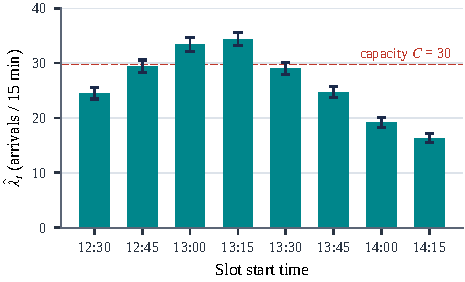
\includegraphics[width=\columnwidth]{rates.pdf}
\caption{Estimated arrival rate per slot with exact 95\% confidence intervals and the capacity $C = 30$.}
\label{fig:rates}
\end{figure}

\begin{figure}[t]
\centering
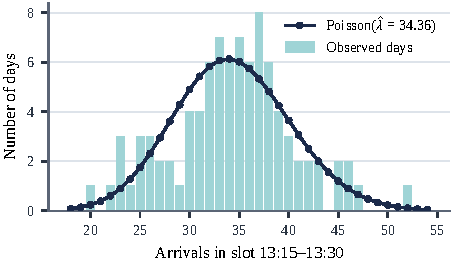
\includegraphics[width=\columnwidth]{gof_peak.pdf}
\caption{Observed distribution of daily counts in the peak slot against the fitted Poisson model.}
\label{fig:gof}
\end{figure}

\begin{table*}[t]
\caption{Per-slot estimates, model checks and overload probabilities ($C = 30$, 40 days)}\label{tab:slots}
\centering\footnotesize
\begin{tabular}{@{}lccccccc@{}}
\toprule
Slot & $\hat\lambda_t$ & 95\% CI & Var/Mean & $\chi^2$ GOF $p$ & $P(X_t > C)$ Poisson, \% & $P(X_t > C)$ Poisson--Gamma, \% & Risk \\
\midrule
\tablerows{generated/table_slots.tex}
\bottomrule
\end{tabular}
\end{table*}

\subsection{Overload risk}
One slot, 12:45--13:00, is high risk ($P = 55.9\%$); 12:30--12:45 ($49.0\%$) and 13:00--13:15 ($30.1\%$) are medium
risk, and no slot is low risk (Fig.~\ref{fig:overload}). Keeping $P(X_t > C)$ below 20\% in every slot would need a
capacity of 36 per slot at the peak, against 30 at present. Once slot and day effects are removed, the Pearson test
finds no extra day-to-day variation ($\chi^2_P = 59.7$ on 111 df; $\hat v = 0$): the counts vary, if anything, less
than a Poisson model allows (dispersion ratio 0.54). The Poisson--Gamma model therefore reduces to the Poisson model and
gives the same overload probabilities.

\begin{figure}[t]
\centering
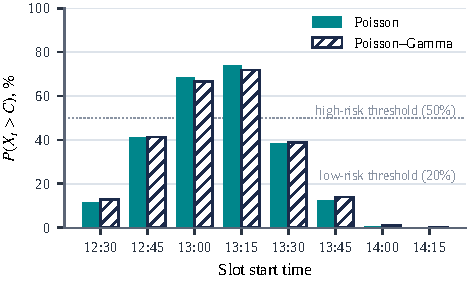
\includegraphics[width=\columnwidth]{overload.pdf}
\caption{Overload probability per slot with the risk thresholds. The Poisson--Gamma bars equal the Poisson bars
because no extra day-to-day variation was found ($\hat v = 0$).}
\label{fig:overload}
\end{figure}

\subsection{Day-specific forecast and peak time}
The regression explains 55.5\% of the variance of log counts (adjusted $R^2 = 0.523$). Relative to Monday, Saturday
multiplies expected arrivals by 0.724 ($t = -6.87$, $p < 0.001$) and Sunday by 0.745 ($t = -6.25$, $p < 0.001$); the
13:00 slot is 9.3\% quieter than 12:30 ($p = 0.002$), and Tuesday to Friday do not differ significantly from Monday
(Table~\ref{tab:coef}). On daily totals the weekdays do not differ (ANOVA $p = 0.371$, Kruskal--Wallis $p = 0.414$),
whereas weekends are clearly quieter (71.0 against 96.2 arrivals over the three slots; Welch $t = -10.21$, $p < 0.001$;
Mann--Whitney $p < 0.001$).

Fig.~\ref{fig:forecast}(a) shows the resulting forecasts. On a regular Monday the probability that at least one slot is
overloaded is 94.9\%, with 1.8 overloaded slots expected; on a Friday 97.4\% and 2.1; on a Saturday only 21.9\% and 0.2.
The peak is most likely at 12:45--13:00 (46\%), with 12:30--12:45 close behind, so the peak falls in 12:30--13:00 with
probability 83\% (Fig.~\ref{fig:forecast}(b)). Neighbouring slots have similar rates, so the peak time is genuinely
uncertain on any single day even when the rates are known.

\begin{table}[t]
\caption{Regression of $\ln(x + 0.5)$ on slot, weekday and day type}\label{tab:coef}
\centering\footnotesize
\setlength{\tabcolsep}{4pt}
\begin{tabular}{@{}lrrrrr@{}}
\toprule
Term & Estimate & SE & $t$ & $p$ & $e^{\hat\beta}$ \\
\midrule
\tablerows{generated/table_coef.tex}
\bottomrule
\end{tabular}\\[2pt]
{\scriptsize $^{\dagger}$Reference levels: slot 12:30, Monday. The weekend day type is captured by the Saturday and
Sunday terms. Slots are labelled by start time.}
\end{table}

\begin{figure*}[t]
\centering
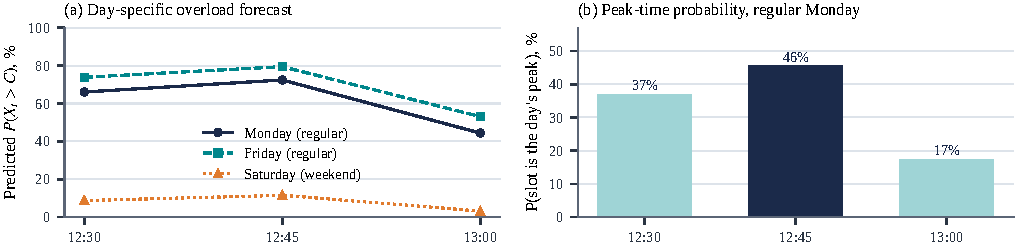
\includegraphics[width=\textwidth]{forecast.pdf}
\caption{(a) Predicted overload probability for a Monday, a Friday and a Saturday. (b) Probability that each slot is
the busiest of the day on a regular Monday, from 20{,}000 simulated lunch periods.}
\label{fig:forecast}
\end{figure*}

\subsection{Same-day update}
Because $\hat v = 0$, the Gamma prior on the day's busyness factor is concentrated at 1, and the counts in the first
slot carry no information about the later slots beyond what the regression already predicts: a first slot 15\% busier
than forecast leaves the 12:45--13:00 overload probability at 72.4\%. On this canteen, a busy start therefore does not
signal a busy rest of lunch; the update would matter only where whole days vary more than Poisson.

\subsection{Validation on unseen days}
Twenty days (60 slot forecasts) were forecast one day ahead. Table~\ref{tab:tests} summarises the tests and
Fig.~\ref{fig:validation} the calibration. The 95\% prediction intervals covered all actual counts, which the $z$-test
does not distinguish from the nominal level ($p = 0.076$). The predicted busiest slot was correct on 60\% of days
against 40\% by chance ($z = 1.83$, $p = 0.034$). Predicted and actual counts correlate with $r = 0.616$
($p < 0.001$). The overload forecasts have a Brier score of 0.172 against 0.248 for the per-slot average, a skill of
31\%. The daily mean absolute error was 3.93 for the model against 4.44 for the average, but the difference is not
significant (paired $t$, $p = 0.111$; sign test 12 of 20 days, $p = 0.252$); the gain comes from weekends (3.26 against
4.81) and Fridays (4.34 against 5.84), which the average cannot tell apart from other days. The PIT values pass the
Kolmogorov--Smirnov test ($p = 0.099$) but not the chi-square test ($p = 0.001$): few values fall near 0 or 1, so the
forecast distributions are somewhat wider than needed, consistent with the counts being less variable than Poisson.
Updating after the first slot leaves the Brier score unchanged (0.181), as expected with $\hat v = 0$.

Within-day carry-over is absent: Spearman correlations of observed-to-predicted ratios between consecutive slots are
$\rho = 0.219$ ($p = 0.17$) and $\rho = -0.086$ ($p = 0.60$). The runs test finds no clustering of busy days (17 runs
against 21.0 expected, $p = 0.20$).

\begin{table*}[t]
\caption{Hypothesis tests of the one-day-ahead forecasts (20 unseen days, 60 slot forecasts, $\alpha = 0.05$)}\label{tab:tests}
\centering\footnotesize
\begin{tabular}{@{}llllll@{}}
\toprule
Check & Test & Statistic & $p$ & Result & Supports the model \\
\midrule
\tablerows{generated/table_tests.tex}
\bottomrule
\end{tabular}
\end{table*}

\begin{figure*}[t]
\centering
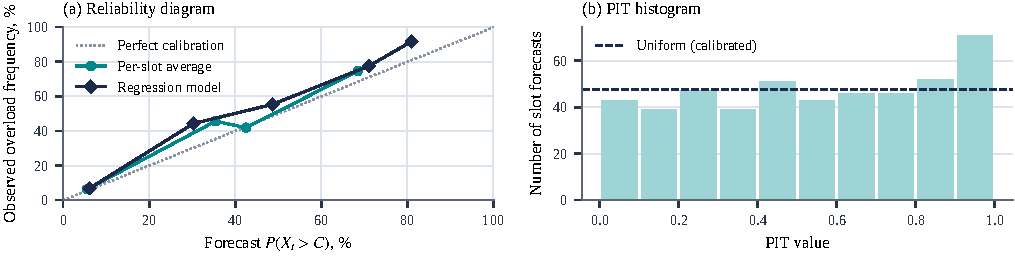
\includegraphics[width=\textwidth]{validation.pdf}
\caption{Calibration on unseen days. (a) Forecast overload probability against observed overload frequency.
(b) Randomised PIT values of the count forecasts; a flat histogram indicates a calibrated forecast distribution.}
\label{fig:validation}
\end{figure*}

% ===================================================================================================
\section{Discussion}\label{sec:discussion}
The per-slot Poisson model fits every slot and turns arrival counts into a direct answer: at this canteen the 15
minutes from 12:45 are overloaded on more than half of all days, and from 13:00 the pressure eases significantly.
Testing the assumption slot by slot, rather than building it in as queueing studies do~\cite{chen2011,yuan2023,jiao2022},
is what makes the probabilities defensible; the pooled Pearson test adds a check that whole days do not vary more than
Poisson, and here they do not.

The forecasting results are mixed and are reported as such. The day-of-week model captures the weekend drop that a
per-slot average misses, which gives its overload forecasts a clear Brier skill and cuts the error on weekends by a third; it
names the peak slot more often than chance, and its intervals contain the actual counts. Its overall point accuracy is
not significantly better than the per-slot average over 20 test days, in line with the observation that simple
fixed-effect models are hard to beat when the remaining day effects are mild~\cite{ibrahim2016}. With no extra
day-to-day variation, the same-day update adds nothing at this canteen.

\textit{Limitations.} (i) The record covers 40 days and only the first 45 minutes of lunch; later slots, exam weeks and
other semesters are not observed. (ii) With 20 test days the validation has limited power. (iii) The model estimates
arrival risk, not queue length, which also depends on service rates and counters. (iv) The rate is assumed constant
within a slot and arrivals independent, whereas groups of friends arrive together. (v) The regression scales a whole
day up or down and cannot move the peak to another slot on special days without slot-by-day interactions. (vi) Least
squares on log counts stands in for Poisson regression. (vii) Capacity and risk thresholds are project decisions that
must be justified for a specific canteen.

% ===================================================================================================
\section{Conclusion and Future Work}\label{sec:conclusion}
This paper estimated the probability that canteen arrivals exceed capacity in each 15-minute slot using a Poisson
model checked slot by slot, and extended it to predict a specific day's risk and peak time. On 40 recorded days the
methods identified 12:45--13:00 as the high-risk slot, a significantly quieter time from 13:00, a capacity of 36 per
slot needed to keep every slot below 20\% risk, a weekend drop of about 26\%, and an 83\% probability that a regular Monday's
peak falls in 12:30--13:00, while showing honestly that the gain in point accuracy over a per-slot average is not
significant on this record.

Future work will extend the counts to the whole lunch period and a full semester including exam weeks, add service
times to estimate queue length through an M/M/$c$ model, model group arrivals with compound Poisson distributions,
estimate a smooth rate $\lambda(t)$~\cite{leemis1991}, and automate counting with turnstile or camera data.

\bibliographystyle{IEEEtran}
\bibliography{references}

\end{document}
